% !TEX root = ../dg.tex

\section{Affine Connections}
\label{sec:connections}

We would like to define geodesics on Riemannian manifolds. These are the analogs of straight lines, in the sense both that they are defined as ``straightest'' paths on Riemannian manifolds and that shortest paths between points are always geodesics. To do so, we will need to define an intrinsic notion of the derivative of a vector field along a curve; then the geodesics will be the curves whose tangent vectors differentiate to zero (just like the tangent vector to a straight line parametrized at constant speed is constant, and hence its derivative is zero; or, if you like, the acceleration along a straight line is zero).

This notion of differentiation will be called the \emph{covariant derivative}. If our manifold is a smooth surface in $\R^3$ (with the Riemannian metric induced by the Euclidean structure on $\R^3$), then there's a simple geometric description of the covariant derivative, which I will now try to explain.

Let $S$ be a smooth surface in $\R^3$ and let $\alpha \from I \to S$ be a smooth curve in $S$, where $I$ is some interval. Suppose $V$ is a vector field along $\alpha$. Concretely, we can write $V \from I \to \R^3$ so that $V(t) \in T_{\alpha(t)}S$: that is, at each $t$, the vector $V(t)$ is tangent to the curve $\alpha$.

In general, there is no reason that $V'(t)$ should be tangent to $S$.

\begin{example} 
	Consider the case where $S$ is the unit sphere, $\alpha(t) = \left(\frac{1}{\sqrt{2}}\cos t, \frac{1}{\sqrt{2}}\sin t, \frac{1}{\sqrt{2}} \right)$ is the circle of latitude at $45^\circ$ North, and 
	\[
		V(t) := \left( \sin^2 t - \frac{1}{\sqrt{2}} \cos^2 t, -\frac{2+\sqrt{2}}{4} \sin 2t, \frac{1}{\sqrt{2}} \cos t\right).
	\]
	See \Cref{fig:curvefield}. 
	
	\begin{figure}[htbp]
		\centering
			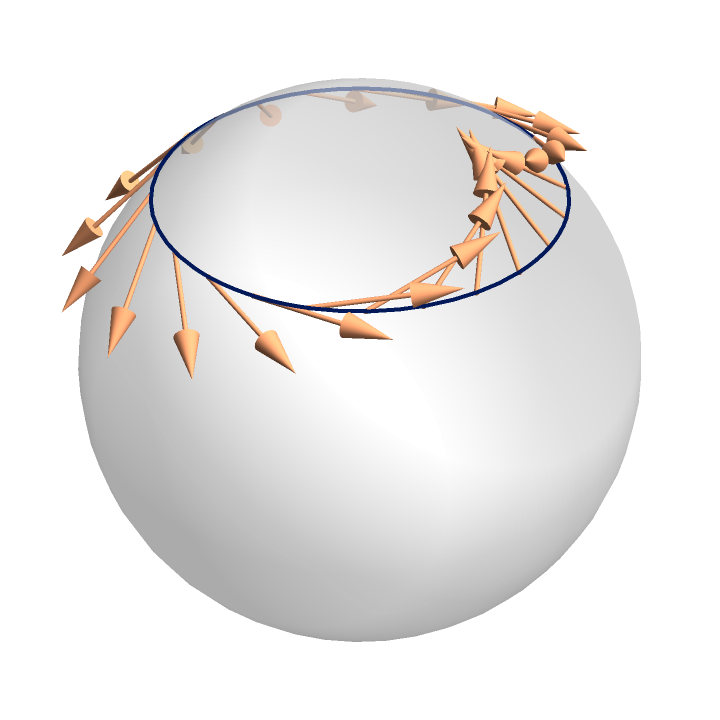
\includegraphics[height=1.5in]{curvefield}
		\caption{The unit sphere with curve $\alpha(t)$ colored in dark blue and the vector field $V(t)$ in orange.}
		\alttext{A sphere viewed from slightly above with curve and vector field as described in the caption and main text.}
		\label{fig:curvefield}
	\end{figure}
	
	Then 
	\[
		V'(t) = \left((2 + \sqrt{2})\cos t \sin t,- \frac{2 + \sqrt{2}}{2}\cos 2t, - \frac{\sin t}{\sqrt{2}}\right).
	\]
	Hence $V'(\pi/2) = \left(0,1+\frac{1}{\sqrt{2}},-\frac{1}{\sqrt{2}}\right)$ is not in the tangent space to $\alpha(\pi/2) = \left(0, \frac{1}{\sqrt{2}},\frac{1}{\sqrt{2}}\right)$ since 
	\[
		V'(\pi/2) \cdot \alpha(\pi/2) = \frac{1}{\sqrt{2}} \neq 0.
	\]
\end{example}

The fact that $V'(t)$ is not generally tangent to $S$ means that $V'(t)$ is not a notion of derivative that can be defined intrinsically to the surface. However, in this case, the simplest possible fix turns out to give something that \emph{is} intrinsically defined. Specifically, we know that $\alpha(t) \in S$, and so we have the tangent space $T_{\alpha(t)}S$ to $S$ at $\alpha(t)$. Of course, $\alpha(t) \in \R^3$ as well, and $\R^3$ has its own tangent space at $\alpha(t)$, namely $T_{\alpha(t)}\R^3$. But then $V'(t) \in T_{\alpha(t)}\R^3$ and $T_{\alpha(t)} S \subset T_{\alpha(t)}\R^3$, so we can orthogonally project $V'(t)$ to $T_{\alpha(t)}S$, as in \Cref{fig:projection}.

\begin{figure}[htbp]
	\centering
		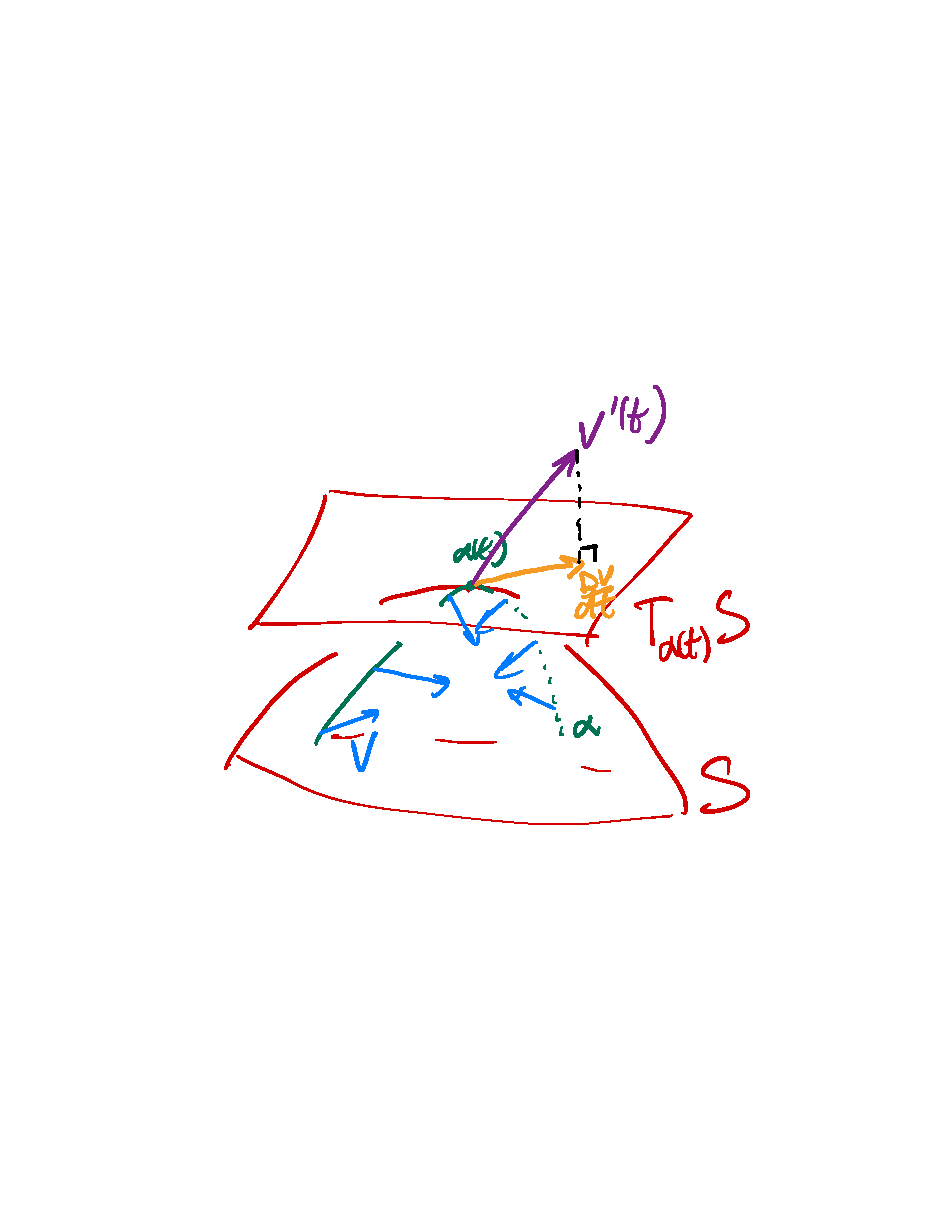
\includegraphics[height=1.5in]{projection}
	\caption{The projection of $V'(t)$ onto $T_{\alpha(t)}S$ yields the covariant derivative $\frac{DV}{dt}$.}
	\alttext{A surface $S$ containing a curve $\alpha$, which has a vector field $V$ along it. At a point $\alpha(t)$ on the curve, $V'(t)$ is orthogonally projected onto $T_{\alpha(t)}S$.}
	\label{fig:projection}
\end{figure}

The projection of $V'(t)$ onto $T_{\alpha(t)}S$ is called the \emph{covariant derivative} of $V$ along $\alpha$ and denoted $\frac{DV}{dt}$. While this still seems extrinsic to the surface, it turns out you can define $\frac{DV}{dt}$ purely in terms of $\alpha$, $V$, $S$, and the Riemannian metric $g$ on $S$. While in this example the Riemannian metric is induced by the Euclidean metric on $\R^3$, you can use the same formula to define $\frac{DV}{dt}$ for \emph{any} Riemannian metric $g$ on a surface, regardless of whether or not $g$ is induced from a Euclidean metric.

In turn, we say that a vector field $V$ along $\alpha$ is \emph{parallel} if $\frac{DV}{dt} \equiv 0$; then a geodesic is just a curve $\alpha$ so that $\alpha'(t)$ is parallel along $\alpha$. 

If you want to see more details on the above, see any standard textbook on curves and surfaces, for example do Carmo's book~\cite{carmoDifferentialGeometryCurves1976} or O'Neill's~\cite{oneillElementaryDifferentialGeometry2006}. Here, I'm going to develop the general theory on arbitrary Riemannian manifolds, which uses a gadget called a \emph{connection}. These can be defined on any manifold (not just Riemannian manifolds), but, as we'll see, a Riemannian metric produces a special connection.

\begin{definition}\label{def:affine connection}
	An \emph{affine connection} $\nabla$ on a manifold $M$ is a mapping
	\[
		\nabla \from \mathfrak{X}(M) \times \mathfrak{X}(M) \to \mathfrak{X}(M)
	\]
	sending $(V,W) \mapsto \nabla_V W$ satisfying the following:
	\begin{enumerate}
		\item \label{it:connection1} Linearity in the first factor: $\nabla_{f_1V_1 + f_2 V_2} W = f_1 \nabla_{V_1}W + f_2 \nabla_{V_2}W$
		\item \label{it:connection2} Additivity in the second factor: $\nabla_V(W_1 + W_2) = \nabla_V W_1 + \nabla_V W_2$
		\item \label{it:connection3} The Leibniz rule in the second factor: $\nabla_V(f W) = V(f) W + f \nabla_V W$.
	\end{enumerate}
\end{definition}

\begin{example}\label{ex:euclidean connection}
	In $\R^n$, suppose $W = \sum_k w_k \frac{\partial}{\partial x_k}$ and define
	\[
		\nabla_V W = \sum_k V(w_k) \frac{\partial}{\partial x_k}.
	\]
\end{example}

\begin{lemma}\label{lem:connection is local}
	Affine connections are local in the sense that the value of $\nabla_V W$ at $p$ depends only on $V(p)$ and the values of $W$ in a neighborhood of $p$.
\end{lemma}

\begin{proof}
	Let $g$ be a smooth function with support in some small neighborhood of $p$, with $g \equiv 1$ on some even smaller neighborhood. Then at $p$ we have $V(g) = 0$, and hence at $p$
	\[
		\nabla_V (g W) = V(g) W + g \nabla_V W = \nabla_V W
	\]
	by \ref{it:connection3}. Since the support of the cutoff function $g$ can be arbitrarily small, we see that $\nabla_V W$ depends only on the values of $W$ in a small neighborhood of $p$.
	
	From \ref{it:connection1}, we know $\nabla_{fV}W = f \nabla_V W$, so it follows immediately that $\nabla_V W$ at $p$ also depends only on the values of $V$ in a neighborhood of $p$.
	
	In fact, we can show more. Let $(U,\phi)$ be a coordinate chart in a neighborhood of $p$ and let $X_1 = \frac{\partial}{\partial X_1}, \dots , X_n = \frac{\partial}{\partial x_n}$ be the coordinate vector fields. If $V = \sum_i v_i X_i$, then
	\[
		\nabla_V W = v_1 \nabla_{X_1} W + \dots + v_n \nabla_{X_n}W
	\]
	by \ref{it:connection1}. If we evaluate the right hand side at $p$, the only dependence on $V$ come from the $v_i(p)$, so it only depends on $V(p)$ (and not on the behavior of $V$ in a neighborhood of $p$).
\end{proof}

If $\nabla$ is an affine connection on $M$ and $X_1 = \frac{\partial}{\partial X_1}, \dots , X_n = \frac{\partial}{\partial x_n}$ in some coordinate neighborhood on $M$, define the smooth functions $\Gamma_{ij}^k$ on that coordinate neighborhood by
\[
	\nabla_{X_i} X_j = \sum_{k} \Gamma_{ij}^k X_k.
\]
The $\Gamma_{ij}^k$ are called the \emph{Christoffel symbols} of the connection $\nabla$, and we can write a formula for $\nabla_V W$ in terms of them: if $V = \sum_i v_i X_i$ and $W = \sum_j w_j X_j$ are vector fields defined on a coordinate neighborhood, then
\begin{align*}
	\nabla_V W & = \sum_i v_i \nabla_{X_i} \left( \sum_j w_j X_j \right) \\
	& = \sum_{i,j}\left( v_i X_i(w_j) X_j + v_i w_j \nabla_{X_i} X_j \right) \\
	& = \sum_{i,j}\left( v_i X_i(w_j) X_j + v_i w_j \sum_k \Gamma_{ij}^k X_k \right) \\
	& = \sum_{i,j,k} \left( v_i X_i(w_k) + v_i w_j \Gamma_{ij}^k \right)X_k \\
	& = \sum_{i,j,k} \left( v_i \frac{\partial w_k}{\partial x_i} + v_i w_j \Gamma_{ij}^k \right)X_k .
\end{align*}

\begin{exercise}\label{ex:christoffel determines connection}
	Show that, within a coordinate neighborhood, if we pick $n^3$ smooth functions $\Gamma_{ij}^k$ arbitrarily and define
	\[
		\nabla_V W := \sum_{i,j,k} \left( v_i \frac{\partial w_k}{\partial x_i} + v_i w_j \Gamma_{ij}^k \right)X_k,
	\]
	then $\nabla$ will satisfy the axioms of an affine connection in that coordinate neighborhood.
\end{exercise}

\begin{remark}
	Despite the suggestive notation, the $\Gamma_{ij}^k$ are not the components of a tensor field on $M$: they do not transform like tensor components under general coordinate transformations.
\end{remark}

We can refine \Cref{lem:connection is local} a bit: we don't actually need to know $W$ on an entire neighborhood of $p$, but only along a curve within that neighborhood:

\begin{lemma}\label{lem:connection is local2}
	The value of $\nabla_V W$ at $p$ depends only on the value of $V$ at $p$ and the value of $W$ along any (short) curve through $p$ which is tangent there to $V(p)$.
\end{lemma}

\begin{proof}
	We've just seen that, in local coordinates,
	\begin{equation}\label{eq:connection local coords}
		\nabla_V W = \sum_{i,j,k} \left( v_i \frac{\partial w_k}{\partial x_i} + v_i w_j \Gamma_{ij}^k \right)X_k = \sum_{i,j,k} \left( V(w_k) + v_i w_j \Gamma_{ij}^k \right)X_k
	\end{equation}
	since $V = \sum_i v_i \frac{\partial }{\partial x_i}$. The only term which is not entirely determined by $V(p)$ and $W(p)$ is $V(w_k) = (\alpha \circ w_k)'(0)$ for some curve $\alpha$ with $\alpha(0) = p$ and $\alpha'(0) = V(p)$. Of course, $(\alpha \circ w_k)(t)$ only depends on the values of $W$ along $\alpha$.
\end{proof}

An affine connection then gives us a way of defining covariant derivatives:

\begin{proposition}\label{prop:covariant derivative}
	Let $\nabla$ be an affine connection on a smooth manifold $M$. Then we can uniquely associate to any vector field $W$ along a curve $\alpha \from I \to M$ another vector field $\frac{DW}{dt}$ along $\alpha$ such that
	\begin{enumerate}
		\item \label{it:cov der1} $\frac{D(W_1 + W_2)}{dt} = \frac{DW_1}{dt} + \frac{DW_2}{dt}$
		\item \label{it:cov der2} $\frac{DgW}{dt} = \frac{dg}{dt} W + g \frac{DW}{dt}$
		\item \label{it:cov der3} If $W$ is defined on all of $M$, then
		\[
			\frac{DW}{dt} = \nabla_{\frac{d\alpha}{dt}} W.
		\]
	\end{enumerate}
\end{proposition}

\begin{definition}\label{def:covariant derivative}
	The vector field $\frac{DW}{dt}$ guaranteed by \Cref{prop:covariant derivative} is called the \emph{covariant derivative} of $W$ along $\alpha$.
\end{definition}

\begin{proof}[Proof of \Cref{prop:covariant derivative}]
	If we work in local coordinates, we have $\alpha(t) = (\alpha_1(t), \dots , \alpha_n(t))$, so
	\[
		\frac{d\alpha}{dt} = \sum_i \frac{d\alpha_i}{dt} X_i,
	\]
	so the formula \eqref{eq:connection local coords} for $\nabla_VW$ shows that we must define
	\begin{equation}\label{eq:covariant derivative def}
		\frac{DW}{dt} := \sum_{i,j,k} \left( \frac{dw_k}{dt} + \frac{d\alpha_i}{dt} w_j \Gamma_{ij}^k \right)X_k
	\end{equation}
	in order to satisfy conditions \ref{it:cov der1}, \ref{it:cov der2}, and \ref{it:cov der3}. Hence, the covariant derivative, if it exists, must  be unique. But to get existence we just define the covariant derivative in coordinates as in \eqref{eq:covariant derivative def}.
\end{proof}

The thing to remember about affine connections is that they give a way of defining parallel transport; that is, some way of moving a tangent vector ``parallel to itself'' along a curve. In general, there's no canonical way to do this, so you have to define what you mean by ``parallel,'' and that's really what a connection does.

\begin{example}
	Consider the unit sphere $S^2 \subset \R^3$ and take the tangent vector $\frac{\partial}{\partial y}$ at the north pole. Say we want to transport this vector parallel to itself around the spherical triangle that traverses a great circle south from $(0,0,1)$ to $(1,0,0)$, then the equator east from $(1,0,0)$ to $(0,1,0)$, and finally another great circle north from $(0,1,0)$ to $(0,0,1)$. If course, we could move $\frac{\partial}{\partial y}$ parallel to itself in $\R^3$, which just gives $\frac{\partial}{\partial y}$ at every point along the curve; see \Cref{fig:sphereparallel1}. But $\frac{\partial}{\partial y}$ is not in the tangent space at $(0,1,0) \in S^2$: it's perpendicular to the sphere at that point!
	
	\begin{figure}[htbp]
		\centering
			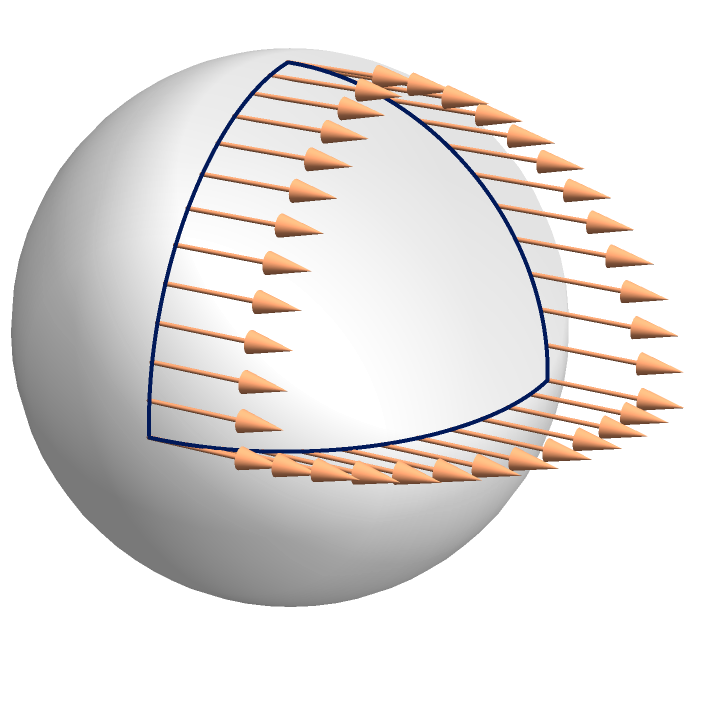
\includegraphics[height=1.5in]{sphereparallel1}
		\caption{Parallel translating a vector around a curve in the ambient space.}
		\alttext{A vector pointing to the right at every point along the spherical triangle described in the main text.}
		\label{fig:sphereparallel1}
	\end{figure}
	
	To get something which stays tangent to the sphere, we simply take the vector field which is always pointing east. Along the first segment, traveling south from the north pole to $(1,0,0)$, this is the same thing we had before. You can imagine a traveler walking south along this path, and then the vector field is just what they get when they stick out their left hand.
	
	At $(1,0,0)$, the traveler turns left, and now east is straight ahead as they start walking toward $(0,1,0)$, so now the vector field is what they get by pointing straight ahead. From the perspective of the traveler, this is the same direction as along the first leg of their journey (namely, east!).
	
	When they arrive at $(0,1,0)$, the traveler now turns left again to face north. Now east is to their right, and they can trace out the vector field by just sticking out their right hand as they walk north. Notice that, once the traveler gets back to the north pole, the vector we get by parallel translating the initial vector around the curve is perpendicular to the initial vector! So even though all along the way the vector field was constant (from the perspective of the traveler or, more mathematically, with respect to the intrinsic geometry of the sphere), it realizes some nontrivial transformation of the initial vector.\footnote{This phenomenon is called \emph{holonomy}, and arises whenever there is curvature.} See \Cref{fig:sphereparallel2}.
	
	\begin{figure}[htbp]
		\centering
			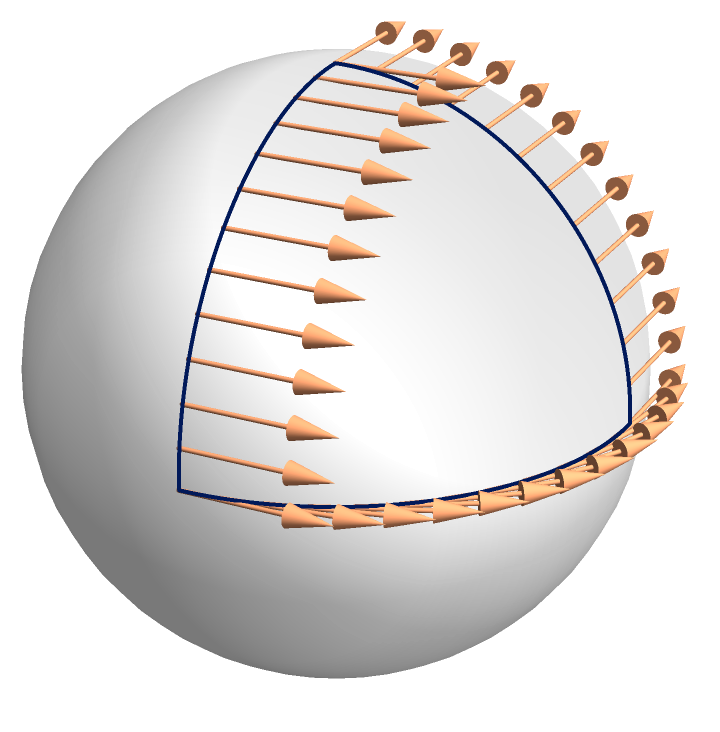
\includegraphics[height=1.5in]{sphereparallel2}
		\caption{Parallel translating a vector around a curve intrinsically.}
		\alttext{A vector pointing to the east at every point along the spherical triangle described in the main text.}
		\label{fig:sphereparallel2}
	\end{figure}
\end{example}

The idea of parallel translation is the same in general: the idea is that, as you traverse a curve, you're not changing the direction of the vector.

\begin{definition}\label{def:parallel vector field}
	Let $M$ be a smooth manifold with affine connection $\nabla$. A vector field $V$ along a curve $\alpha \from I \to M$ is \emph{parallel} (along $\alpha$) if $\frac{DV}{dt} = 0$ for all $t \in I$.
\end{definition}

\begin{example}
	With respect to the standard connection $\nabla$ on $\R^n$ from \Cref{ex:euclidean connection}, a vector field $V = \sum_i v_i \frac{\partial}{\partial x_i}$ is parallel (along any curve) if and only if the $v_i$ are constants. The $V$ shown in \Cref{fig:sphereparallel1} is an example if you just think of the curve as a curve in $\R^3$ and ignore the sphere.
\end{example}

It turns out that, given any initial vector at a point and any curve through the point, we can always find a parallel field along the curve which agrees with the given vector at the point.

\begin{proposition}\label{prop:parallel transport}
	Let $M$ be a smooth manifold with an affine connection $\nabla$, let $\alpha \from I \to M$ be a smooth curve in $M$, and let $V_0 \in T_{\alpha(t_0)}M$ be some tangent vector to $M$ at $\alpha(t_0)$. Then there is a unique parallel vector field $V \from I \to TM$ along $\alpha$ so that $V(t) \in T_{\alpha(t)}M$ for all $t \in I$ and $V(t_0) = V_0$.
\end{proposition}

\begin{proof}
	In local coordinates, the parallel condition $\frac{DV}{dt} = 0$ is a system of $n$ first order linear ODEs for the coefficients of $V$. Then the standard existence and uniqueness theorems apply and we get a unique solution with given initial condition.
\end{proof}

\begin{definition}\label{def:parallel transport}
	The vector field $V(t)$ guaranteed by \Cref{prop:parallel transport} is called the \emph{parallel transport} of $V_0 = V(t_0)$ along the curve $\alpha(t)$.
\end{definition}

From here, we could define geodesics, curvatures, etc. for arbitrary connections. Rather than develop this theory in full generality, we will specialize to the case of the \emph{Riemannian connection} or \emph{Levi-Civita connection}, which is uniquely determined by a Riemannian metric. So we turn to the task of defining this special connection.